%\pagestyle{fancy}
\chapter{Results}
\label{ch:Results}

\section{Evaluation concept}
\todoin{\begin{itemize}
		\item The straight ramp on floor -2 will be used as main example
		\item All plots will be only made for that ramp
		\item Except maybe for special edge cases (e.g. influence of braking on imu estimation)
		\item All the other ramps will be only evaluated using scores, displayed in tables
	\end{itemize}}
To prevent an overfitting of the model, it is important to have many test scenarios.
Six different ramps will be tested, some of which will be driven up and some down.
An additional recording without any ramp was made to test false positives.
As mentioned in \cref{ch:ExperimentalSetup}, the wheel odometer measurements are only available, when the motor output of the car is limited.
This means that recordings with the odometer data were only possible for the test cases, where the car is driving down or only halfway up.



\section{Ramp metering? (\glsentrytext{imu})}
To evaluate the performance of the different algorithms, a reference must be used.
The most accurate one available is the one produced by the \texttt{hdl\_graph\_slam}~\footnote{\url{https://github.com/koide3/hdl_graph_slam}} package.
This package is based on 3D graph slam and uses the \gls{lidar} data to estimate the position and orientation.
Because the \gls{lidar} only records at \SI{10}{\hertz} and the other sensors record from \SIrange{100}{400}{\hertz}, the estimate was upsampled using a Fourier method.\\
The goodness of the fit between the estimated road grade $\hat{y} = (\hat{y}_i, \dots, \hat{y}_n)^\intercal$ and the reference $y = (y_i, \dots, y_n)^\intercal$ can be described by the \gls{rmse}
\begin{equation}
	RMSE = \sqrt{\frac{1}{n}\sum_{i = 1}^n(\hat{y}_i - y_i)^2},
\end{equation}
which quantifies how much the predicted values differ from the reference value on average.
It is defined in the range $[0, \infty)$, with a value of 0 indicating a perfect fit.
Furthermore, the coefficient of determination $R^2$ is used
\begin{equation}
	R^2 = 1 - \frac{\sum\limits_{i = 1}^n(\hat{y}_i - y_i)^2}{\sum\limits_{i = 1}^n(\hat{y}_i - \overline{y})^2},
\end{equation}
where $\overline{y}$ indicates the mean of the reference.
The goodness of the fit is described in the range from 0 to 1, where 1 describes a perfect fit.\\
Different recordings of different ramps were made, but the results will be discussed on only two test drives.
In the first drive the car was accelerated from stand still and drove up ramp A \todo{Picture and label of every ramp in setup section} about half-way up.
As explained in ?, the ramp could not be driven completely, due to the need of the odometer readings, which are only available when the motor output is limited.
\begin{figure}[htbp]
	\centering
	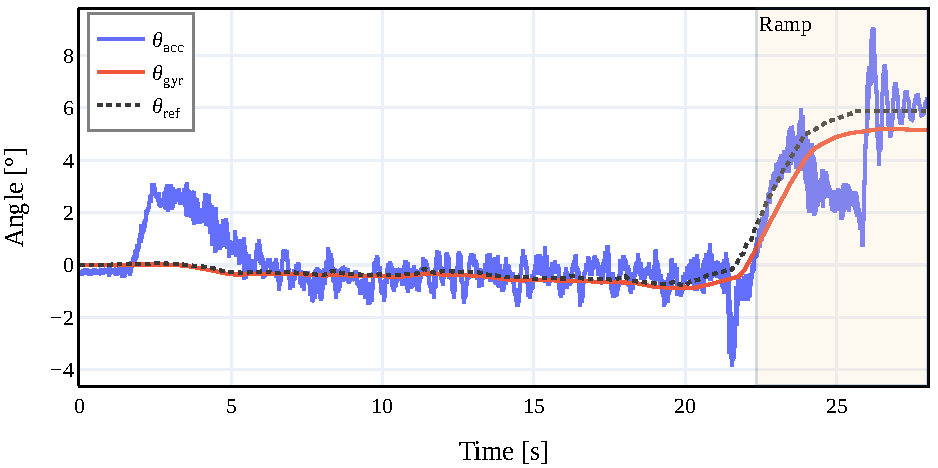
\includegraphics[width=.9\linewidth]{imu_raw_angle.pdf}
	\caption[Raw]{Pitch angle calculated from the raw accelerometer and gyroscope measurements}
	\label{fig:imu_raw_angle}
\end{figure}
The result of using only the raw measurements of the \gls{imu} for the pitch calculation is shown in \cref{fig:imu_raw_angle}.
The accelerometer is very noisy and is easily influenced by accelerations other than gravity, which can be seen at \SIrange{2}{4}{\second}, where the car started driving.
The gyroscope on the other hand provides good short-term accuracy and is not influenced by other accelerations, but is slowly drifting over time.\\
\iimprov{Show another plot of a longer drive, where drift is even more apparent}
The gravity method tries to overcome the problem of the accelerometer of also detecting other accelerations than gravity, by subtracting the car's acceleration from the accelerometer measurement.
The car's acceleration $\vb{a}_\mathrm{odom,x} $ was calculated by calculating the derivate of the low-pass filtered car velocity $v_\mathrm{car} $, which was calculated from the wheel speed measurements according to REF.
Figure \ref{fig:imu_odometer_acc} shows the (low-pass filtered) acceleration measured by the \gls{imu} along the x-axis and the (low-pass filtered) car's acceleration.
$\vb{a}_\mathrm{grav,x} $ is the acceleration measured by the \gls{imu} from which the car acceleration $\vb{a}_\mathrm{odom,x} $ was subtracted.
It can be seen, that especially at the beginning of the ramp (\SIrange{21}{23}{\second}) the gravity method shows it advantages.
The deceleration before entering the ramp is measured by both sensors and thus cancels out each other.
The same can be seen in the initial acceleration phase, where the car starts to drive from still stand (\SIrange[]{2}{4}{\second}).
Although both sensor are synchronized in time, the \gls{imu} senses the acceleration earlier than the wheel speed sensors which leads to a slight pike.
This could be due to the wheel speed sensors having a certain velocity threshold, below which they do not pick up any changes.
Other reasons for the difference could be, that other forces than the one from the car are present, e.g. from the suspension of the car or vibrations due to the road quality, which were not taken into account.
Also the approximations made by calculating the finite difference of the car velocity to get the car acceleration have a negative influence on the result.
\itodo{Either here or in methods: Describe problem with deriv car velocity $\to$ filtering beforehand was necessary}
\begin{figure}[htbp]
	\centering
	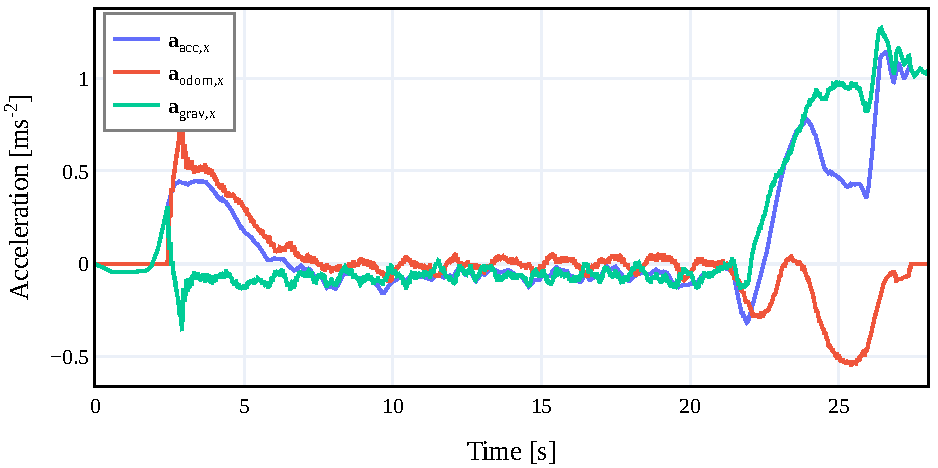
\includegraphics[width=.9\linewidth]{imu_odometer_acc.pdf}
	\caption[Acceleration from \gls{imu} and odometer]{Measured acceleration in x-direction by the \gls{imu} and acceleration derived from the wheel speed measurements and the difference between both}
	\label{fig:imu_odometer_acc}
\end{figure}
The resulting angle from the acceleration can be seen in \cref{fig:imu_odometer_angle}.
The reference is taken from the orientation estimation of the \texttt{hdl\_graph\_slam}, which uses the \gls{lidar} data.
It can be seen that the gravity method improves the estimation accuracy significantly, compared to when only using the accelerometer data.
Especially the angle at the start and on the ramp is more accurately described when adding the odometer data to the accelerometer data for the calculation.
But it can also be seen that the time synchronization between both signals is vital, as seen in during the initial acceleration phase.
\begin{figure}[htbp]
	\centering
	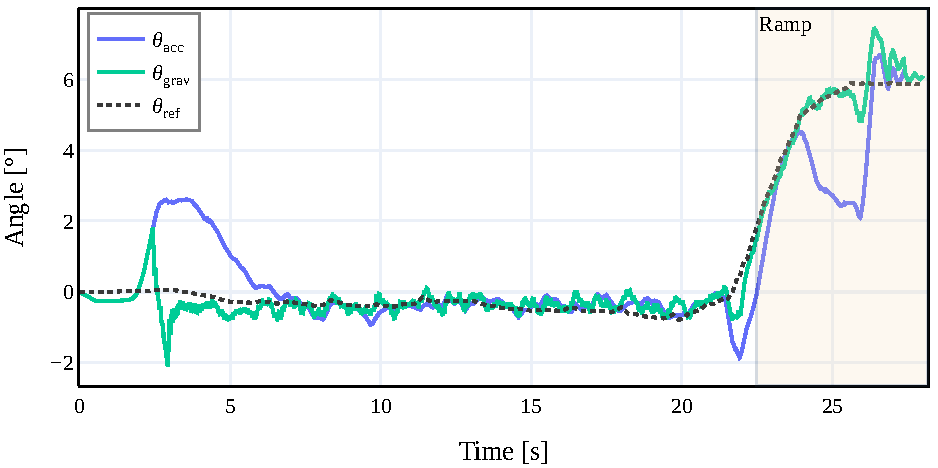
\includegraphics[width=.9\linewidth]{imu_odometer_angle.pdf}
	\caption[Gravity method]{The road grade estimation using only the accelerometer compared to the gravity method, which additionally uses the wheel speed measurements}
	\label{fig:imu_odometer_angle}
\end{figure}
Another way to improve the estimation is using a complementary filter, as shown in \cref{fig:imu_raw_compl_angle}.
The complementary filter uses the estimation of the gyroscope measurements and corrects them using the accelerometer measurements to prevent drift.
It can be seen that the estimation using the complementary filter closely follows the reference except for the .. between the two ramps.
SOMETHING MORE
\begin{figure}[htb]
	\centering
	\begin{subfigure}{1\textwidth}
		\centering
		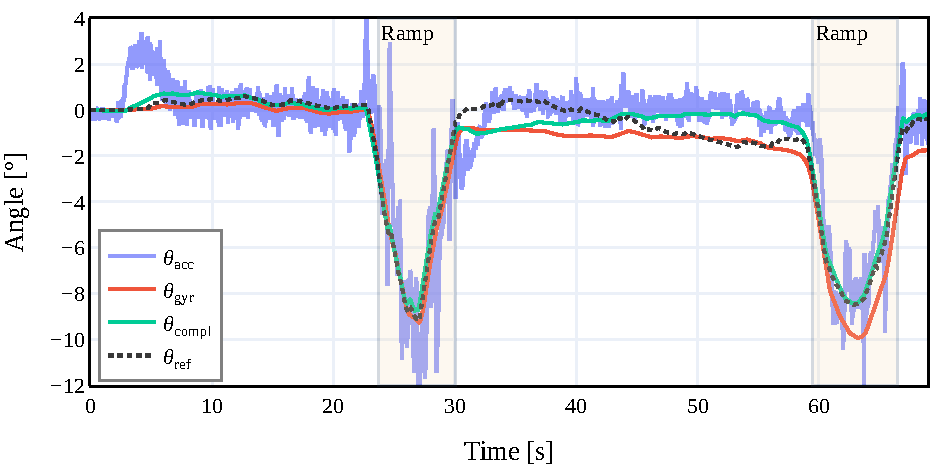
\includegraphics[width=0.9\linewidth]{imu_raw_compl_angle.pdf}
		\caption{Complementary filter}
		\label{fig:imu_raw_compl_angle}
	\end{subfigure}
	
	% \bigskip
	\begin{subfigure}{1\textwidth}
		\centering
		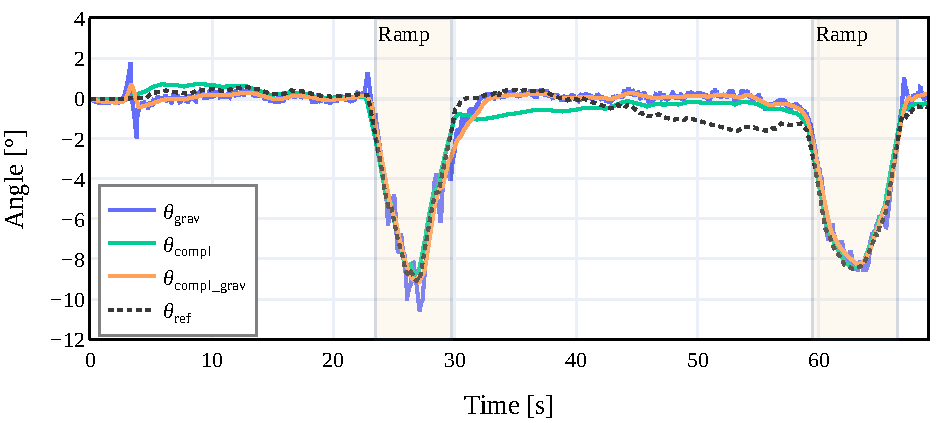
\includegraphics[width=0.9\linewidth]{imu_grav_compl_angle.pdf}
		\caption{Something other ($\theta_\mathrm{compl, grav}$ is the same as compl and $\theta_\mathrm{grav}$ is just filtered acc)}
		\label{fig:imu_grav_compl_angle}
	\end{subfigure}
	\caption{This bag clearly shows the drift of the gyro, but lacks odometer measurements}
\end{figure}
\missingfigure{Plot of different compl gains}
\missingfigure{Plot of problem of distance estimation using only accelerometer (initial acc is bad)}
\todoin{\begin{itemize}
		\item Think of better way to split test drives (e.g. up, down and long and short)
		\item Tune parameters
		\item Ignore acc odom if no odom has been recorded
		\item Add distance measurement (for full drives)
		\item Add angle estimate (final estimate)
		\item Possible add delay for acc odom and compl methods (due to lowpass filtering)
	\end{itemize}}

\begin{table}[htbp]
	\centering
	\caption{Performance evaluation zed}
	\label{tab:eval_table}
	\begin{tabular}[t]{cccccccccc}
		\toprule
		\textbf{Properties} & \multicolumn{3}{c}{\textbf{Uphill short}} & \multicolumn{3}{c}{\textbf{Uphill long}} & \multicolumn{3}{c}{\textbf{Downhill long}}                                                                                                     \\
		\midrule
		Mean(v)             & \multicolumn{3}{c}{5}                     & \multicolumn{3}{c}{5}                    & \multicolumn{3}{c}{5}                                                                                                                          \\
		Max(v)              & \multicolumn{3}{c}{7}                     & \multicolumn{3}{c}{3}                    & \multicolumn{3}{c}{9}                                                                                                                          \\
		Angle               & \multicolumn{3}{c}{7}                     & \multicolumn{3}{c}{3}                    & \multicolumn{3}{c}{9}                                                                                                                          \\
		\hline
		\textbf{Method}     & \textbf{RMSE}                             & $\mathbf{R^2}$                           & \textbf{angle}                             & \textbf{RMSE} & $\mathbf{R^2}$ & \textbf{angle} & \textbf{RMSE} & $\mathbf{R^2}$ & \textbf{angle} \\
		Acc                 & 0.7                                       & 0.5                                      & 7                                          & 0.5           & 0.7            & 8              & 0.5           & 0.7            & -5             \\
		Gyr                 & 0.7                                       & 0.5                                      & 7                                          & 0.5           & 0.7            & 8              & 0.5           & 0.7            & -5             \\
		
		\bottomrule
	\end{tabular}
\end{table}

\begin{table}[htbp]
	\centering
	\caption{Performance evaluation zed}
	\label{tab:eval_table}
	\begin{tabular}[t]{cccccccc}
		\toprule
		\textbf{Structure} & \textbf{Method} & \textbf{RMSE} & $\mathbf{R^2}$ & \textbf{Delay?} \\
		\midrule
		uc                 & acc             & 0.93          & 0.75           & ?               \\
		uc                 & acc odom        & 0.72          & 0.87           & ?               \\
		uc                 & compl           & 0.68          & 0.88           & ?               \\
		uc                 & compl grav      & 0.68          & 0.88           & ?               \\
		uc                 & gyr             & 1.42          & 0.51           & ?               \\
		us                 & acc             & 1.11          & 0.67           & ?               \\
		us                 & acc odom        & 0.84          & 0.81           & ?               \\
		us                 & compl           & 0.80          & 0.83           & ?               \\
		us                 & compl grav      & 0.80          & 0.83           & ?               \\
		us                 & gyr             & 0.47          & 0.93           & ?               \\
		\bottomrule
	\end{tabular}
\end{table}

\begin{table}[htbp]
	\centering
	\caption{Performance evaluation myahrs}
	\label{tab:eval_table}
	\begin{tabular}[t]{cccccccc}
		\toprule
		\textbf{Structure} & \textbf{Method} & \textbf{RMSE} & $\mathbf{R^2}$ & \textbf{Delay?} \\
		\midrule
		uc                 & acc             & 0.85          & 0.79           & ?               \\
		uc                 & acc odom        & 0.70          & 0.88           & ?               \\
		uc                 & compl           & 0.69          & 0.89           & ?               \\
		uc                 & compl grav      & 0.69          & 0.89           & ?               \\
		uc                 & gyr             & 1.42          & 0.14           & ?               \\
		us                 & acc             & 0.99          & 0.73           & ?               \\
		us                 & acc odom        & 0.79          & 0.84           & ?               \\
		us                 & compl           & 0.76          & 0.86           & ?               \\
		us                 & compl grav      & 0.76          & 0.86           & ?               \\
		us                 & gyr             & 0.44          & 0.95           & ?               \\
		\bottomrule
	\end{tabular}
\end{table}
\todoin{\begin{itemize}
		\item How well do different \gls{imu} methods work...
		\item ... at ramp detection
		\item ... at ramp distance measuring
		\item ... at angle estimation
	\end{itemize}}
\todo[inline, caption={2do}, color=green!40]{
	\begin{minipage}{\textwidth-4pt}
		\begin{itemize}
			\item Which methods should be compared?
			\item Because gravity method only works with odometer, which is only available when driving down or halfway up
			\item Should new recording at different offset angles be made?
			\item How to handle false positives, e.g. when braking on level ground?
			\item What to display in the table, only normal drives or also ones with braking etc.?
			\item Or evaluate those edge cases separately? (Probably with plot of est angle)
			\item How to handle offline vs live detection (for the offline detection the measurements can be butterworth filtered)?
			\item How to determine the delay of the detection (using the camera image)?
			\item What about the consistency test recordings, how or where to display the results?
		\end{itemize}
	\end{minipage}
}
\isug{Raw accelerometer data or gyroscope peak is ramp start}
\isug{Also show consistency recordings (avg error and stuff)}
\todoin{\begin{itemize}
		\item Plots of (all only for one ramp)...
		\item Acceleration from \gls{imu} and odometer (already filtered)
		\item Angle estimation using only lin acc, ang vel
		\item Angle estimation comparing different sophisticated methods (complementary, gravity etc.)
		\item Plot comparing angle estimation using the different \gls{imu}s
	\end{itemize}}




\section{Ramp detection (\glsentrytext{lidar} and camera)}
rmse[] = distance, angle and width

\begin{table}[htbp]
	\centering
	\caption{Performance evaluation}
	\label{tab:eval_table}
	\begin{tabular}[t]{cccccccc}
		\toprule
		\textbf{Structure} & \textbf{Distance}        & \textbf{Frames} & \textbf{TP} & \textbf{FP} & \textbf{rmse1}    & \textbf{rmse2}     & \textbf{rmse3}    \\
		\midrule
		uc                 & \SIrange{0}{5}{\metre}   & 62              & 100.00\%    & 0.00\%      & \SI{0.75}{\metre} & \SI{0.61}{\degree} & \SI{0.75}{\metre} \\
		uc                 & \SIrange{5}{10}{\metre}  & 62              & 100.00\%    & 0.00\%      & \SI{0.84}{\metre} & \SI{0.68}{\degree} & \SI{0.84}{\metre} \\
		uc                 & \SIrange{10}{15}{\metre} & 59              & 100.00\%    & 0.00\%      & \SI{0.89}{\metre} & \SI{0.60}{\degree} & \SI{0.89}{\metre} \\
		uc                 & \SIrange{15}{20}{\metre} & 61              & 97.92\%     & 2.08\%      & \SI{2.75}{\metre} & \SI{0.95}{\degree} & \SI{2.75}{\metre} \\
		uc                 & \SIrange{20}{25}{\metre} & 61              & 97.83\%     & 2.17\%      & \SI{3.69}{\metre} & \SI{0.94}{\degree} & \SI{3.69}{\metre} \\
		uc                 & \SIrange{25}{30}{\metre} & 59              & 42.75\%     & 0.00\%      & \SI{2.36}{\metre} & \SI{2.22}{\degree} & \SI{2.36}{\metre} \\
		us                 & \SIrange{0}{5}{\metre}   & 162             & 83.33\%     & 6.67\%      & \SI{3.83}{\metre} & \SI{0.85}{\degree} & \SI{3.83}{\metre} \\
		us                 & \SIrange{5}{10}{\metre}  & 149             & 83.33\%     & 0.00\%      & \SI{0.75}{\metre} & \SI{0.41}{\degree} & \SI{0.75}{\metre} \\
		us                 & \SIrange{10}{15}{\metre} & 144             & 100.00\%    & 0.00\%      & \SI{0.76}{\metre} & \SI{0.37}{\degree} & \SI{0.76}{\metre} \\
		us                 & \SIrange{15}{20}{\metre} & 150             & 87.41\%     & 0.74\%      & \SI{1.38}{\metre} & \SI{0.52}{\degree} & \SI{1.38}{\metre} \\
		us                 & \SIrange{20}{25}{\metre} & 169             & 79.38\%     & 0.69\%      & \SI{5.62}{\metre} & \SI{1.22}{\degree} & \SI{5.62}{\metre} \\
		us                 & \SIrange{25}{30}{\metre} & 78              & 43.42\%     & 0.00\%      & \SI{1.73}{\metre} & \SI{1.65}{\degree} & \SI{1.73}{\metre} \\
		\bottomrule
	\end{tabular}
\end{table}

% Option1	Structure	Dist interval	TP	FP
% 	Straight up
% 	Straight down
% 	Straight down at 90
% 	Curved up
% 	Curved down

% Option2	Structure	Offset angle	Distance	Frames	TP	FP

% Option3	Structure	StdDev/mean/var etc of distance, angle, width and length
\todoin{\begin{itemize}
		\item Confusion matrix or similar (false negatives could be hard (e.g. curve))
		\item Estimated angle and distance compare to ground truth
		\item Do downwards ramp work?
		\item Camera \gls{lidar} projection for nice visualization
		\item Something about camera
	\end{itemize}}
\itodo{Make new recordings of level -2 ramps, approaching at different (e.g. 0, 15, 30, 45) angles}

\todo[inline, caption={2do}, color=green!40]{
	\begin{minipage}{\textwidth-4pt}
		\begin{itemize}
			\item Should structure be only one ramp (and direction) or should it include multiple?
			\item How to choose distance interval?
			\item What about offset angle?
			\item What about estimated distance, angle, width and length?
			\item What is a true positive? (E.g. some detected points lie in region, or at least $x$\% lie in region, or less than $y$\% points lie outside\dots)
			\item Are number of frames important?
			\item I've done multiple recordings of e.g. straight ramp on -2 floor, but only one of the ones on floor -1, how to handle?
		\end{itemize}
	\end{minipage}
}
\isug{Anzahl Fahrten als Spalte}
\isug{Subcategories rampentyp}
\begin{figure}[htbp]
	\centering
	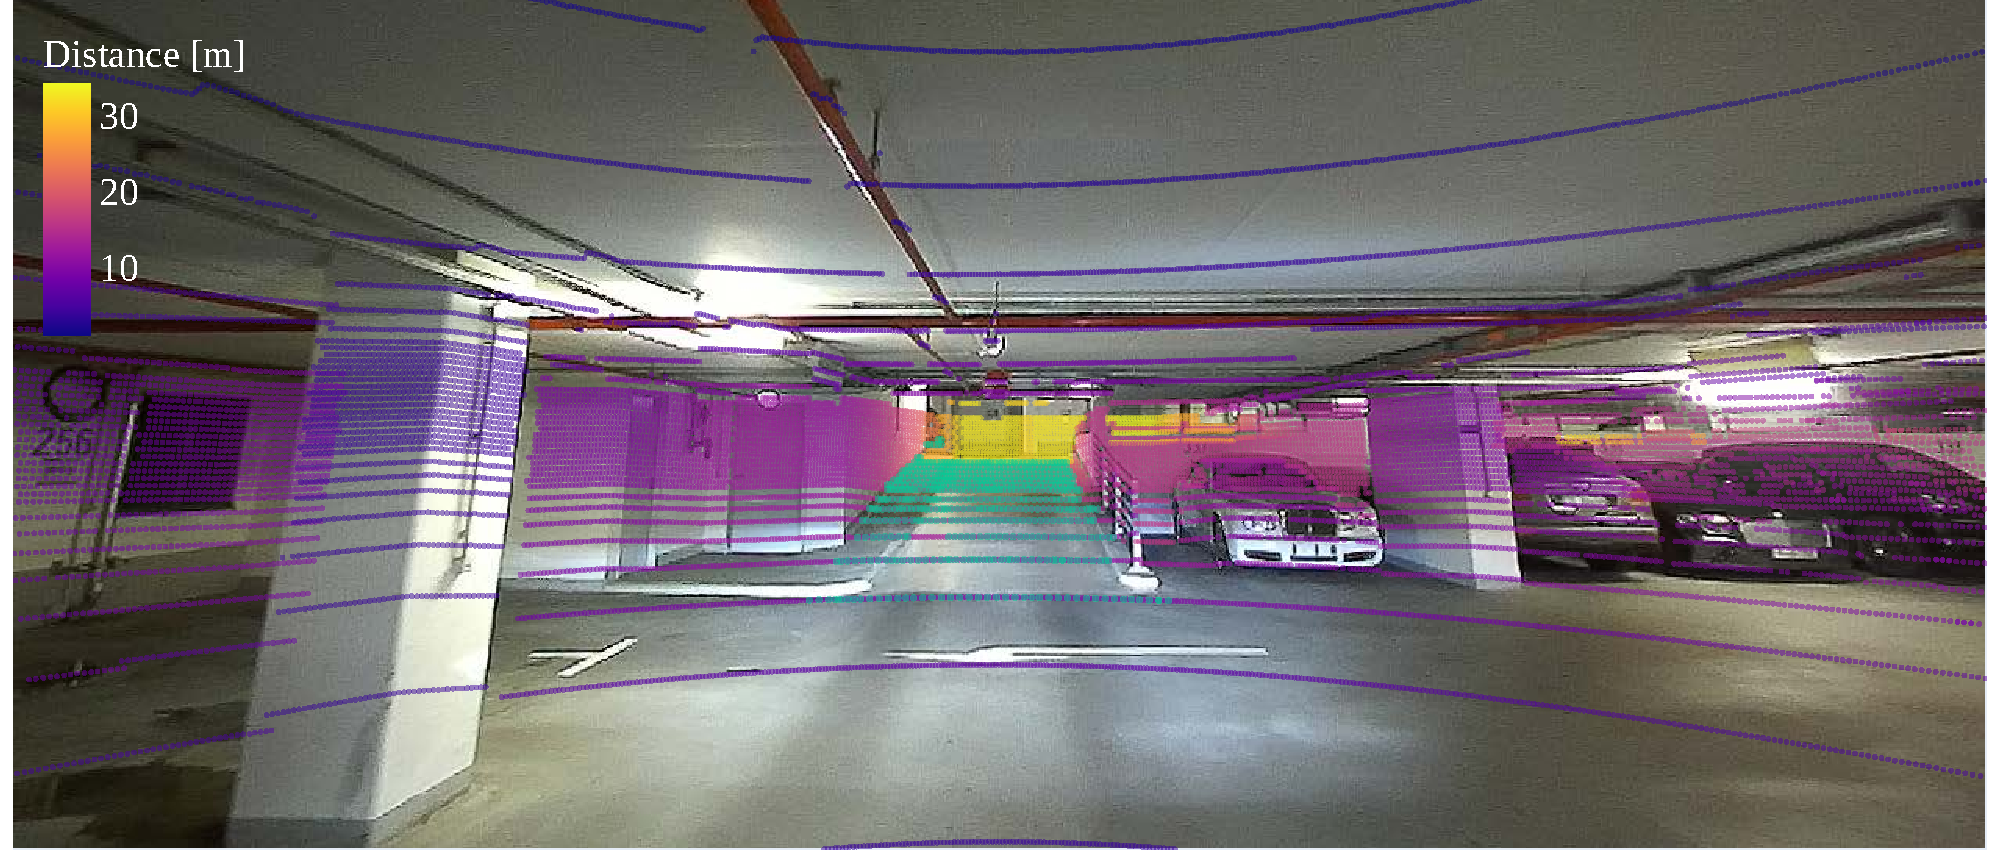
\includegraphics[width=1\linewidth]{points_projection.pdf}
	\caption{Lidar points projected into the camera image. The green points were identified as part of a ramp.}
\end{figure}
\newpage
\begin{figure}[htbp]
	\centering
	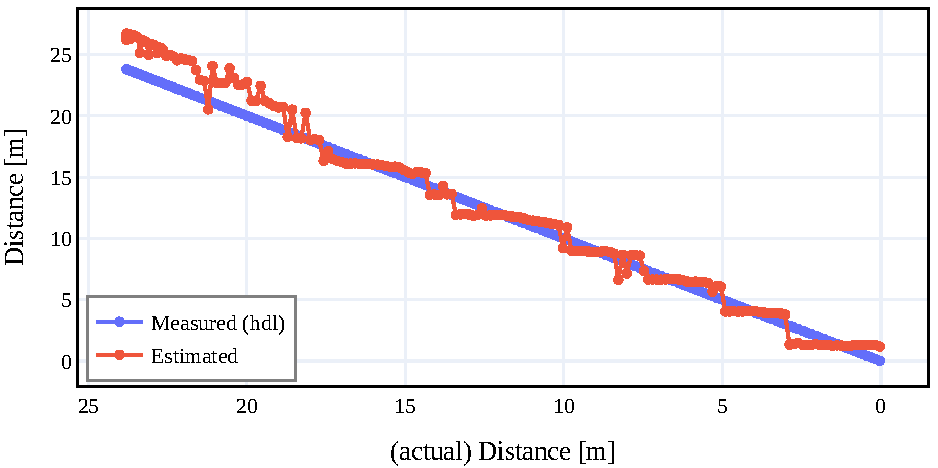
\includegraphics[width=0.7\linewidth]{lidar_distance_eval.pdf}
	\caption{Difference between estimated and measured distance to ramp}
	\label{fig:lidar_distance_eval}
\end{figure}
\begin{figure}[htbp]
	\centering
	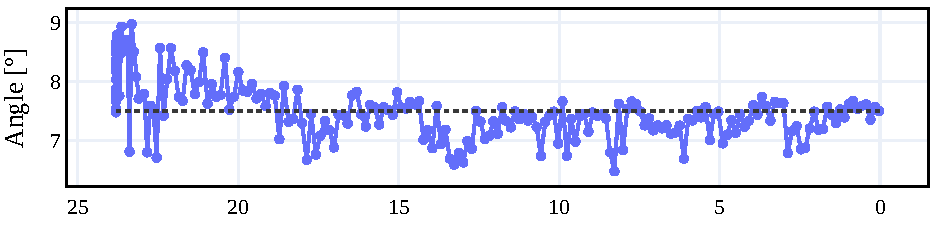
\includegraphics[width=0.7\linewidth]{lidar_angle_eval.pdf}
	\caption{Error between estimated and measured ramp angle (\SI{6.75}{\degree})}
	\label{fig:lidar_angle_eval}
\end{figure}
\begin{figure}[htbp]
	\centering
	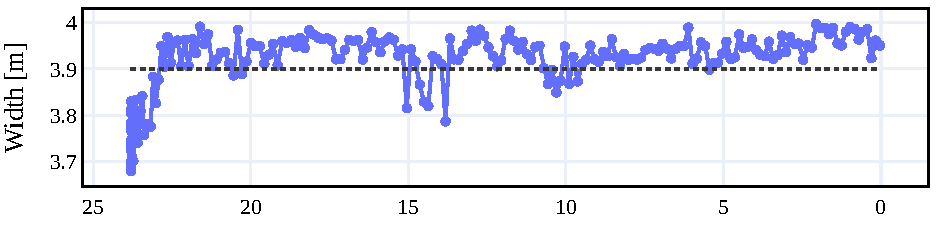
\includegraphics[width=0.7\linewidth]{lidar_width_eval.pdf}
	\caption{Error between estimated and measured ramp width (\SI{4}{\metre})}
	\label{fig:lidar_width_eval}
\end{figure}

\begin{figure}[htb]
	\centering
	\begin{subfigure}{1\textwidth}
		\centering
		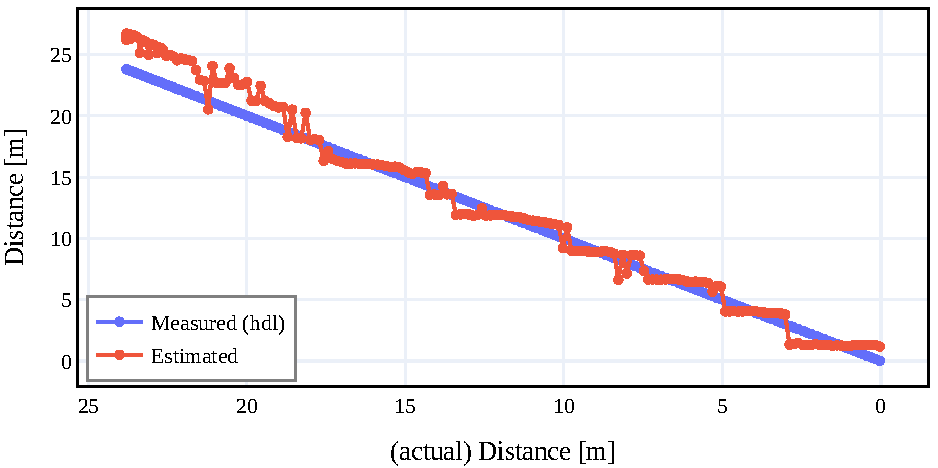
\includegraphics[width=0.7\linewidth]{lidar_distance_eval.pdf}
		\caption{caption}
		\label{fig:lidar_distance_evalTest}
	\end{subfigure}
	
	% \bigskip
	\begin{subfigure}{1\textwidth}
		\centering
		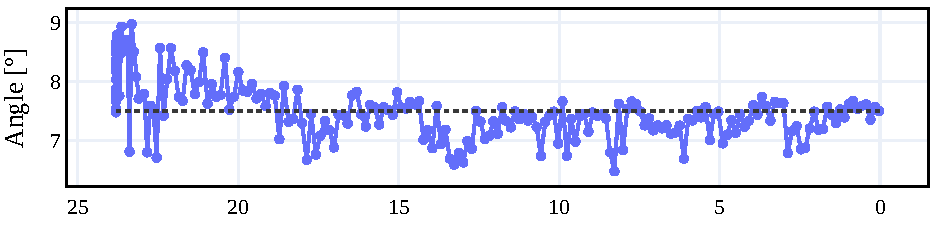
\includegraphics[width=0.7\linewidth]{lidar_angle_eval.pdf}
		\caption{caption}
		\label{fig:lidar_angle_evalTest}
	\end{subfigure}
	
	\begin{subfigure}{1\textwidth}
		\centering
		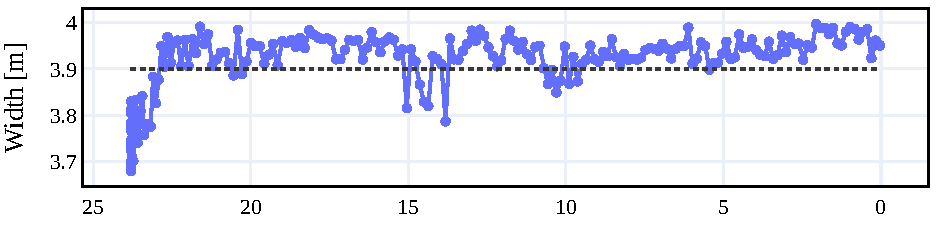
\includegraphics[width=0.7\linewidth]{lidar_width_eval.pdf}
		\caption{caption}
		\label{fig:lidar_width_evalTest}
	\end{subfigure}
	\caption{Is subfigure better than separate?}
	\label{fig:subFigTest}
\end{figure}

\begin{figure}[htbp]
	\centering
	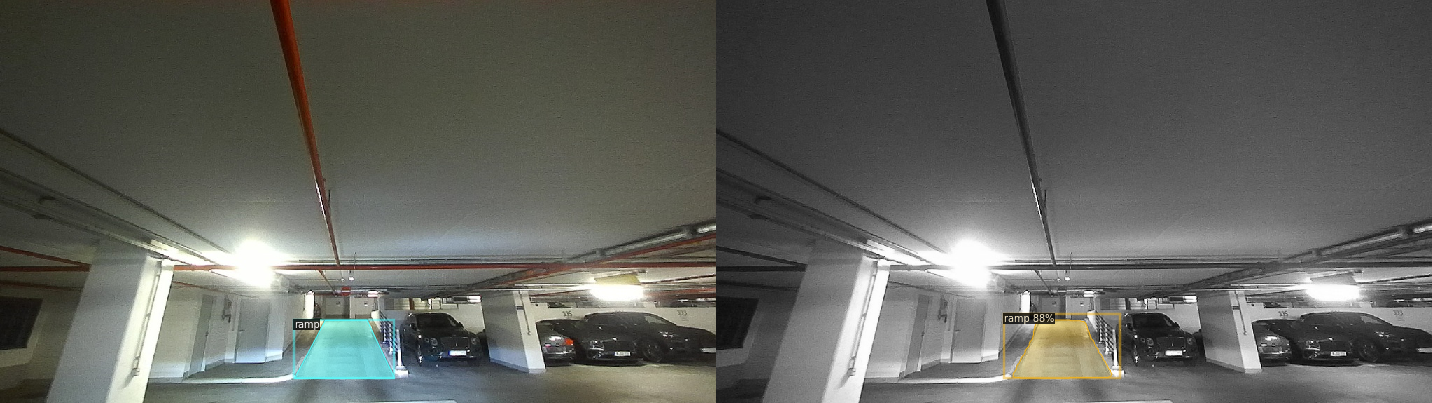
\includegraphics[width=1\linewidth]{camera_detection_compare}
	\caption{Machine learning}
	\label{fig:camera_detection_compare}
\end{figure}